\documentclass[journal,12pt,twocolumn]{IEEEtran}
\usepackage{setspace}
\usepackage{gensymb}
\usepackage{caption}
\usepackage{hyperref}
\usepackage{graphicx}
\usepackage{tabularx}
\usepackage{lmodern}
\usepackage{watermark}
\usepackage{karnaugh-map} 
\usepackage{lipsum}
\usepackage{xcolor}
\usepackage{listings}

\title{BOOLEAN LOGIC}
\author{prasad deva}

\begin{document}

\maketitle

\section{problem}
The boolean logic realized by the logic circuit is

\begin{figure}[h]
    \centering
    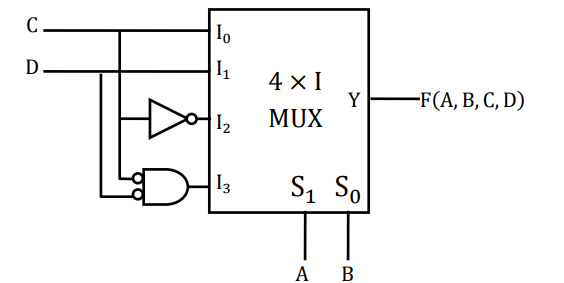
\includegraphics[scale=0.5]{img1.png}
    
    \caption{cbgg}

\end{figure}
\bigskip

\section{COMPONENTS}
\begin{table}[ht!]
    \centering
    \begin{tabular}{|c|c|}
    \hline
         ARDUINO& 1  \\
         \hline
         BREAD BOARD& 1 \\
         \hline
         JUMPER WIRES M-M& 20  \\
         \hline
         7447IC& 1 \\
         \hline
   SEVENSEGMENT DISPLAY& 1 \\
   \hline
RESISTOR& 1 \\
\hline
    \end{tabular}
    \caption{}
\end{table}

\begin{table}[h]
    \setlength{\arrayrulewidth}{0.1mm}
\setlength{\tabcolsep}{18pt}
    \centering
\begin{tabular}{|c|c|c|c|c|c|}
  \hline
    \textbf S.NO &\textbf A &\textbf B &\textbf C & \textbf D &\textbf F  \\
       \hline
     1&0&0&0&0&0 \\
     \hline
     2&0&0&0&1&0 \\
     \hline
     3&0&0&1&0&1 \\
     \hline
     4&0&0&1&1&1 \\
     \hline
     5&0&1&0&0&0 \\
     \hline
     6&0&1&0&1&1 \\
     \hline
     7&0&1&1&0&0 \\
     \hline
     8&0&1&1&1&1 \\
     \hline
     9&1&0&0&0&1 \\
     \hline
     10&1&0&0&1&1 \\
     \hline
     11&1&0&1&0&0 \\
     \hline
     12&1&0&1&1&0 \\
     \hline
     13&1&1&0&0&1 \\
     \hline
     14&1&1&0&1&1 \\
     \hline
     15&1&1&1&0&1 \\
     \hline
     16&1&1&1&1&0 \\
       \hline
\end{tabular}
\caption{Truth Table}
\end{table}
\bigskip

\section{LOGIC}
The logic is writen in the in the form
\bigskip

$ \bar A \bar B I0 + \bar ABI1 + A \bar B I2 + ABI3 $
\bigskip 

$I0 = \bar A \bar B ;$ 
$I1 = \bar AB ;$
$I2 = A \bar B ;$
$I3 = AB $
\bigskip
\begin{table}[h]
\setlength{\arrayrulewidth}{0.3mm}
\setlength{\tabcolsep}{10pt}
  \centering
\begin{tabular}{|c|c|c|}
\hline
\textbf A& \textbf B& \textbf Y \\
\hline
     0&0&C  \\
\hline
     0&1&D \\
\hline
     1&0&$\bar C $\\
\hline
     1&1&$\bar C \bar D $ \\
\hline
\end{tabular}
\end{table} 
\bigskip

\section{karnaugh-map}
The equations to be solved by using the truth table
\bigskip

D) $F = \sum(2,3,5,7,8,9,12,13,14)$
\bigskip

 \begin{center}
    \begin{karnaugh-map}[4][4][1][$CD$][$AB$] 
   \minterms{2,3,5,7,8,9,12,13,14} 
    \maxterms{0,1,4,6,10,11,15}
    \implicant{3}{2}
    \implicant{5}{7}
    \implicant{12}{9}
    \implicantedge{12}{12}{14}{14}
    \end{karnaugh-map}
    \end{center}
    
    \begin{center}
        TABLE-2: K-map 
    \end{center}
The equation expressed as the TABLE-2
\bigskip

$F = A \bar C + \bar ABD + \bar A \bar BC + AB\bar D$
\bigskip


\section{ARDUINO CONNECTIONS}
 
1)The 7447IC to 7 segment display connections as per the given below table-3
\begin{table}[ht!]
    \centering
    \begin{tabular}{|c|c|c|c|c|c|c|c|}
    \hline
       7447& $\bar a$&$\bar b$&$\bar c$&$\bar d$&$\bar e$&$\bar f$&$\bar g  $ \\
       \hline
    DISPLAY& a&b&c&d&e&f&g \\
    \hline
    \end{tabular}
    \caption{}
\end{table}
\bigskip

2)The 7447IC to arduino connections as per the given below table-4
\begin{table}[ht!]
    \centering
    \begin{tabular}{|c|c|c|c|c|}
    \hline
         7447&A&B&C&D  \\
         \hline
         ARDUINO&2&3&4&5 \\
         \hline
    \end{tabular}
\caption{}
\end{table}
\bigskip

\section{CODE}
The code download by using the below link
\begin{lstlisting}
https://github.com/prasaddeva287/FWC/tree/main/ASSEMBLY/CODES
\end{lstlisting}

\end{document}
 
